\newcommand{\fit}[2]{coeff}

\chapter{Nearby Star-Forming Galaxies in the Mid- and Far-Infrared}
\label{ch:kiss}

\section{Introduction}

In an effort to refine existing metrics of star-formation rate, I present an analysis of mid- and far-infrared photometry of 85 low-redshift H$\alpha$-bright star-forming galaxies detected by the KPNO International Spectroscopic Survey  \citep[KISS;][]{KISSI}, also reported in \cite{Young1}. Because H$\alpha$ selection is not biased toward continuum-bright objects, the KISS sample spans a wide range of stellar masses ($10^8$--$10^{12}\rm{M}_\odot$), H$\alpha$ luminosities ($10^{39}$--$10^{43}\rm{erg/s}$), mid-infrared 8.0$\mu$m luminosities ($10^{41}$--$10^{44}\rm{erg/s}$), and [Bw-R] colors (1.0--2.4). Far-infrared luminosity in Spitzer MIPS bandpasses and mid-infrared polycyclic aromatic hydrocarbon (PAH) emission in Spitzer IRAC bandpasses indicate star formation. I improve empirical calibrations of two such bandpasses, IRAC 8.0$\mu$m and MIPS 24$\mu$m, as indicators of star-formation rate by fitting galactic luminosities in these bands against H$\alpha$-derived extinction-corrected star-formation rates from the KISS sample, and find correlations that are broadly consistent with earlier work. I use novel multiwavelength data to find a strong, color-independent correlation between stellar mass and IRAC 3.6\micron luminosity. Using this surrogate for stellar mass, I measure mass-specific star-formation rates and find that [3.6$\mu$m]-[24$\mu$m] color may be used as a specific star-formation rate indicator, but [3.6$\mu$m]-[8.0$\mu$m] color shows at best a tenuous relationship with specific star-formation rate. Finally, I calibrate a mass dependence in the efficiency of 8.0$\mu$m luminosity as a star-formation rate indicator.

\section{Observations}
\label{sec:kissobs}

\subsection{KISS H$\alpha$-Selected Sample}

The KISS field I focus on in this work is located in the NOAO Deep Wide Field Survey \citep[NDWFS;][]{Jannuzi} in Bo\"{o}tes \citep{Jangren}. The KISS objects were selected from objective-prism spectra to have redshifts $<$ 0.095 and H$\alpha$ emission 5$\sigma$ above their median spectral continua. Objective-prism spectra are preferable to slit spectra for estimating total H$\alpha$ luminosity for extended objects because they capture all of the flux from the object rather than the small fraction that would fall on a slit. A redshift (volume) limit rather than a magnitude limit ensures that the sample is not biased toward galaxies that are intrinsically bright in the continuum. One consideration of volume-limited H$\alpha$ surveys is a bias toward low extinction, however, as mentioned above, this bias makes extinction correction in the H$\alpha$ measurements less of a concern.

In the KISS Bo\"{o}tes field, 131 H$\alpha$ emission line objects were identified. The initial detections were followed up with higher resolution spectroscopy using the Hobby Eberly Telescope (HET), the KPNO 2.1 meter, the MDM 2.4 meter, and the Lick 3 meter telescopes \citep{Wegner,KISSG,Melbourne,KISSV,Salzer}. Using the higher resolution spectra, 28 AGN and LINER galaxies were rejected through an extinction-corrected \ionl{N}{2}{6583}/H$\alpha$ versus \ionl{O}{3}{5007}/H$\beta$ line diagnostic diagram \citep{Baldwin1977,Veilleux1987}. Even though AGN hosts may be sites of star-forming activity, we are unable to disentangle AGN H$\alpha$ emission from that of star-forming activity, making the SFR measurement from such a galaxy unreliable. The 98 remaining objects are the sample from which this study is drawn. Metal abundance estimates were computed for all galaxies using emission-line ratios of strong lines by employing the coarse abundance method described in \cite{MelbourneSalzer} and \cite{Salzer_Metal}. The H$\alpha$ luminosities referenced in this paper shall hereafter refer to H$\alpha$ luminosities that are measured from objective-prism data and are extinction-corrected using reddening estimates from follow-up spectra. 

The greatest uncertainty in this calculation is the extinction correction. The objective-prism H$\alpha$ measurements are used to compute SFRs for the objects in this study because the objective-prism spectra encompass all of the light from the target. However, the Balmer Decrement ($\rm{c}_{\rm{H}\beta}$) measurements from the follow-up spectra represent the extinction averaged over only the regions encompassed by the slit used in the follow-up spectra.  Thus, this uncertainty has a systematic component in that, for objects of large angular size, where only a smaller fraction of the object was encompassed in the slit, the correction applied is more likely to deviate from the true value.  To take this into account, the uncertainties in the H$\alpha$ measurements were weighted by the inverse of the angular size of their respective galaxies.

\subsection{H$\alpha$ Star-Formation Rates}

To calibrate mid- and far-infrared broadband photometry as star-formation rate indicators, I use extinction-corrected H$\alpha$ luminosity as a benchmark indicator. Because the stars contributing with any significance to the ionizing flux have short lifetimes ($<$ 20 Myr), extinction-corrected H$\alpha$ luminosity is an indicator of current star formation and is relatively independent of star-formation history. \cite{Kennicutt} provides an H$\alpha$ luminosity to SFR calibration using solar abundances and a Salpeter IMF (0.1 - 100 M$_\odot$):

\begin{eqnarray}
\rm{SFR}\left[\rm{M}_\odot/yr\right] = 7.9\times10^{-42}\rm{L}_{\rm{H}\alpha}\left[\rm{erg}/\rm{s}\right]\\
\rm{log}\left(\rm{SFR}\left[\rm{M}_\odot/yr\right]\right) = -7.517+\rm{log}\left(\rm{L}_{\rm{H}\alpha}\left[L_\odot\right]\right)
\end{eqnarray}

%The greatest uncertainty in this calculation is the extinction correction itself. The objective-prism H$\alpha$ measurements are used to compute SFRs for the objects in this study because the objective-prism spectra encompass all the light from the target. However, the Balmer Decrement ($\rm{c}_{\rm{H}\beta}$) measurements from the follow-up spectra represent the extinction averaged over only the regions encompassed by the slit used in the follow-up spectra.

Other works, such as \cite{Calzetti2007}, study extinguished H$\alpha$ luminosity in linear combination with mid- or far-infrared luminosity. While extinguished H$\alpha$ samples the ultraviolet luminosity that is unabsorbed by dust, infrared indicators complement extinguished H$\alpha$ because they sample the ultraviolet luminosity that is absorbed by dust. With the proper calibration, a linear combination of the two can estimate total SFR as a sum of extinguished and unextinguished SFRs.

Because of the exquisite follow-up spectra available for this diverse sample of objects, I chose to use H$\alpha$ measurements corrected for extinction 
through the comparison of Balmer decrements to lab measured values, thereby turning the H$\alpha$ measurements into estimates of total SFR, both extinguished and unextinguished. I then use these total SFRs to evaluate mid- and far-infrared luminosities as indicators of total SFR.


\subsection{Spitzer}

The Spitzer data used in this project came from the Spitzer Deep Wide-Field Survey \citep{SDWFS} and The Spitzer Program to Observe the NDWFS Field in Bo\"{o}tes (Soifer et al. 2004).  Spitzer IRAC\footnotemark[6] 3.6$\mu$m, IRAC 4.5$\mu$m, IRAC 5.8$\mu$m, and IRAC 8.0$\mu$m mosaics from the Spitzer Deep Wide-Field Survey cover 86 of the 98 KISS star-forming galaxies; I detect 84 of these galaxies. \footnotetext[6]{IRAC Data Handbook: http://ssc.spitzer.caltech.edu/irac/dh/}The archival MIPS data from Soifer et al. (2004) provides this project with archival Spitzer MIPS\footnotemark[7] 24$\mu$m band coverage for 81 KISS star-forming galaxies; 79 are detected. Although MIPS 70$\mu$m and MIPS 160$\mu$m imaging exists for the KISS galaxies, the object-to-noise contrast is such that the detection rate is less than fifty percent in these bands.  As a result, discussion of MIPS 70$\mu$m and MIPS 160$\mu$m photometry is not included in this work.

\footnotetext[7]{MIPS Data Handbook: http://ssc.spitzer.caltech.edu/mips/dh/}

While photometry in all four IRAC bands and the MIPS 24$\mu$m band is tabulated in Table \ref{phot}, I focus on IRAC 3.6$\mu$m, IRAC 8.0$\mu$m, and MIPS 24$\mu$m because of their relevance to star formation studies. Luminosity in the IRAC 8.0$\mu$m band comes from a combination of sources \citep{Wu}. The primary contributors in the IRAC 8.0$\mu$m band are vibrational emission lines of PAHs and the thermal tail of the old stellar population. Luminosity in the MIPS 24$\mu$m band, on the other hand, samples only thermal dust \citep{Wu}. The IRAC 3.6$\mu$m band is believed to sample primarily the thermal tail of the old stellar population. By studying these fluxes in tandem, I distinguish these different sources of luminosity and provide better calibrated SFR indicators. The IRAC 4.5\micron and 5.8\micron bands are less useful for this particular purpose because they contain weaker PAH bands and more contamination from the stellar continuum than the 8.0\micron band.

While similar research has been conducted previously \citep{Rosenberg,Calzetti2007,Calzetti2010,Wu,AlonsoHerrero,PerezGonzalez}, never before has such a statistically representative population been studied over so diverse a range of wavelengths and in tandem with high-resolution optical spectra. Moreover, unlike other studies sampling small regions within galaxies \citep{Calzetti2005,PerezGonzalez}, the objective-prism spectra ensure that KISS SFRs are global SFRs and can be directly compared to integrated broadband SFR indicator candidates, such as IRAC 8.0$\mu$m and MIPS 24$\mu$m luminosities.

The Spitzer Deep Wide-Field Survey provides IRAC mosaics that are calibrated, co-added, and science ready.  For the MIPS 24$\mu$m photometry I used archival Post Basic Calibrated Data mosaics. Typically, 2-4 Spitzer MIPS observations exist for each object, although a small number have only one observation. I co-added these observations to construct postage-stamp images after aligning them with centroiding software from the NOAO Image Reduction and Analysis Facility (IRAF), and then performed photometry using apertures adjusted by hand to encompass each object simultaneously in the IRAC 3.6\micron and 8.0\micron and MIPS 24\micron images.  The aperture radii ranged from 8\arcsec to 91\arcsec with an average of 19\arcsec. Because the KISS galaxies are extended sources, I performed no aperture corrections.

This method of aperture determination has the significant advantage over automated methods that I was able to encompass unusually and irregularly shaped objects while still excluding nearby objects.  Additionally, because the wavelength scale differs by almost a factor of ten between MIPS 24\micron and IRAC 3.6\micron, most automated methods would have difficulty with the varying PSF scales. As a check, I compared the IRAC magnitudes determined with this method to those listed in the catalog in \cite{SDWFS}; typically, they were within two tenths of a magnitude.

\subsection{NDWFS Optical Imaging}\label{optical}

Because the KISS Bo\"{o}tes field was chosen to overlap with the heavily studied NDWFS Bo\"{o}tes field \citep{Jannuzi}, deep optical images exist for the majority of the KISS galaxies in the Bo\"{o}tes field.  In particular, this study makes use of Bw, R, and I band data for 79 of the 98 star-forming galaxies to calculate stellar masses for these galaxies using well-known mass-to-light relations \citep{Bell}, with which I calibrate 3.6$\mu$m luminosity as a stellar mass indicator.

I performed photometry on these images using the same apertures that were used for photometry on the Spitzer IRAC and MIPS images.  In some cases, the apertures needed to be re-tuned because the higher angular resolution of the NDWFS images revealed nearby contaminating objects, such as foreground stars and other galaxies, which were blended with a KISS galaxy in the Spitzer images.  In these cases, I repeated the Spitzer photometry with the aperture adjusted to avoid the contamination.

Because the KISS galaxies are emission-line selected, emission lines potentially contribute a fair fraction of the light measured in the broadband optical photometry. This is problematic for my study because the mass-to-light relations in \cite{Bell} only apply to light from stellar populations. To remove the emission-line contamination from the broad-band photometry, I scaled the H$\alpha$ equivalent widths measured in the object prism spectra along with the equivalent widths for H$\beta$, \ionl{S}{2}{6717}, \ionl{N}{2}{6583}, \ionl{O}{2}{3727}, and \ionl{O}{3}{5007} lines measured in follow-up spectra \citep{KISSIV,KISSG} by the filter transmission at the redshifted wavelength of their respective lines, and then subtracted their contributions from the Bw and R band photometry.



\section{Analysis}
\label{sec:kissanalysis}

\subsection{Mid- and Far-Infrared Correlations with Total SFR}
\label{direct}



Because PAH features dominate non-stellar 8.0$\mu$m flux by more than a factor of 100 above warm dust emission, and nearly a factor of 10 above the stellar continuum \citep[][see their Figures 8 and 10]{Dale,LiDraine}, 8.0$\mu$m luminosity by itself ought to act as a SFR indicator \citep[e.g.,][]{Calzetti2007}. To calibrate 8.0$\mu$m luminosity as an indicator, I used extinction-corrected H$\alpha$ luminosity as a reference indicator. 

Figure \figref{simple}{a} plots H$\alpha$-measured SFR against 8.0$\mu$m luminosity for the KISS galaxies that have 8.0$\mu$m measurements, along with an error-weighted linear regression determined using the method described in \cite{AkritasBershady}. The points have been color coded for $\LOG{O/H}+12$ metallicity when available from follow-up spectroscopy; a color key is to the right of the plot. The strength of this simple yet direct method of SFR estimation can clearly be seen. 

There is, however, significant contamination from the red tail of the late-type stellar continuum in the 8.0$\mu$m bandpass. Because SED models \citep{LiDraine} indicate that the IRAC 3.6$\mu$m bandpass samples the old stellar population almost exclusively, a dust-only 8.0$\mu$m luminosity can be created by using the 3.6$\mu$m luminosity to estimate and remove the stellar contribution in the 8.0$\mu$m band. As in \cite{Helou}, I adopt a coefficient $\beta$ with a value of 0.232 to be the ratio of the stellar luminosity in the 8.0$\mu$m band to the stellar luminosity in the 3.6$\mu$m band. This ratio is derived from the Starburst99 model \citep{Leitherer}, and as the stellar SED in the mid-infrared regime is not a strong function of stellar age, it is likely to be a reasonable approximation. The dust-only 8.0$\mu$m luminosity shall henceforth be referred to as 8.0$\mu$m (dust). This technique is also used in other work \citep{Calzetti2007,PerezGonzalez,Rosenberg,Wu}, although the adopted value of $\beta$ differs between authors, 0.22-0.29 in \citet{Calzetti2007} and 0.26 in \cite{Wu}, for instance. Figure \figref{simple}{b} plots SFR against 8.0$\mu$m (dust), along with line of best fit. The fitted empirical relations are:

%\begin{equation}
%\rm{log}\left(SFR\left[M_\odot\,yr^{-1}\right]\right) = \left(-7.48\pm0.49\right) + \left(0.832\pm0.054\right)\times \rm{log}\left(L_{8.0\mu m}\left[L_\odot\right]\right)
%\end{equation}
%\begin{equation}
%\rm{log}\left(SFR\left[M_\odot\,yr^{-1}\right]\right) = \left(-7.48\pm0.51\right) + \left(0.836\pm0.056\right)\times \rm{log}\left(L_{8.0\mu m}(dust)\left[L_\odot\right]\right)
%\end{equation}

\begin{equation}
\SFR = \fit{sfr_8micron}{ada} + \fit{sfr_8micron}{bdb}\times \logL{8.0\mu m})
\end{equation}
%\SFR = \left(-7.48\pm0.49\right) + \left(0.832\pm0.054\right)\times \logL{8.0\mu m})
\begin{equation}
\SFR = \fit{sfr_8micron_dust}{ada} + \fit{sfr_8micron_dust}{bdb}\times \logL{8.0\mu m(dust)}
\end{equation}

I list the fitted coefficients for these relations in Table \ref{calibration}, along with the analogous coefficients from other work \citep{Wu,PerezGonzalez}. Although different authors generally agree on the exponential coefficient for this relationship, typically giving it a value around 0.8--0.9, there is great disparity in the linear coefficient. It should be noted that the samples were collected by fairly different means. \cite{Wu} use a magnitude-limited sample favoring large galaxies. They note this, and mention that if several dwarf galaxies had been included in their fit, the slope of their relation would have been different---closer to the one found in this work. \cite{PerezGonzalez} fit their relations to HII regions in M81, but PAH emission may be sensitive to filling factors and other physical effects that would make whole galaxy relations differ from relations based on individual HII regions. The filling factor phenomenon, as well as other physical explanations for problems with PAH emission as a direct SFR indicator, are discussed below. I note that the greater intrinsic scatter of my data, expected from a more uniform sample selection method, results in over a decade of variance in this relation.

Alternatively, some works \citep{AlonsoHerrero,PerezGonzalez,Calzetti2005} conclude that 24$\mu$m far-infrared thermal dust emission correlates with ionizing photons both on the galactic scale and on the scale of star-forming complexes. This band is longward of stellar emission, thus avoiding the somewhat model-dependent correction needed when examining 8.0$\mu$m luminosity. I plot in Figure \figref{simple}{c} extinction-corrected H$\alpha$ SFR against 24$\mu$m luminosities for 81 KISS galaxies, along with a line of best fit. The best fit is:

\begin{equation}
\SFR = \fit{sfr_24micron}{bdb} + \fit{sfr_24micron}{bdb}\times \logL{24\mu m}
\end{equation}

I chose not to use a piecewise indicator because these data do not unambiguously indicate any breaks in the luminosity relation seen in other work \citep[][etc.]{Wu,Calzetti2010}, possibly due to the greater intrinsic scatter in the KISS sample (as discussed below).  Additionally, \cite{Calzetti2010} point out that one motivation for a piecewise indicator is the Luminous Infrared Galaxy (LIRG) mode of star formation at the high luminosity end ( $\rm{L}_{24\mu\rm{m}}\gtrsim  5\times10^{43}\rm{erg/s}$); this volume-limited sample has no LIRGs and only four objects with luminosities in this range, making a piecewise relation with a break at this luminosity both unwarranted and impossible to constrain in this study.

While there this relationship has over a decade of intrinsic scatter, the correlation holds over three decades in 24$\mu$m luminosity. Nevertheless, I note that the relations I described involving 24$\mu$m luminosity can only be expected to apply over the range of 24$\mu$m luminosities studied here ($10^{40}$ to $7.5\times10^{43}$erg/s).

%The exponential coefficient for this relation is 18$\%$ greater than the average of the others listed in Table \ref{calibration}. Independent work \citep{Wu,Calzetti2007,PerezGonzalez,Relano,AlonsoHerrero} all converge on the same linear relation (in log-log space) between 24$\mu$m luminosity and SFR, even when fitted with galaxies or HII regions. 



\subsection{Masses of KISS Galaxies}
\label{masses_of_kiss_galaxies}

The correlations presented above are promising, but without greater insight into the nature of the galaxies being plotted it is unclear if they can be used as reliable SFR indicators for different kinds of galaxies across a range of redshifts. In particular, the total luminosity of a galaxy in any given band depends heavily on how large it is; a more massive galaxy will, on average, be brighter in all bands than a less massive galaxy. This is particularly problematic when trying to calibrate observational relations because even if the causal relationship between SFR and mid- and far-infrared luminosity did not exist, one might still expect the data described in the previous subsections to correlate with each other simply because larger galaxies are statistically more likely to be bright in H$\alpha$ as well as in the mid- and far-infrared bands. 

To this end, I measured the stellar masses of the KISS galaxies using well-established mass-to-light ratios \citep{Bell}. Using galactic stellar masses, I report mass-specific quantities in Section \ref{sec:specific}. The mass-to-light ratios in \cite{Bell} that I used are based on Sloan Digital Sky Survey photometry and population synthesis models. Using I band photometry from NDWFS data \citep{Jannuzi}, I write the logarithmic stellar mass of a galaxy as its logarithmic I band luminosity plus a linear function of [B-R] color:
\begin{equation}
\rm{log}\left({\cal M}\left[M_\odot\right]\right) = \rm{log}\left(L_I\left[L_\odot\right]\right) -0.405 + 0.518\times[B-R],
\end{equation}
I note here that \cite{Bell} report that their optical mass-to-light relations have an uncertainty of $\sim0.1$ dex, and that I have propagated this uncertainty forward through the equations that follow.

Figure \ref{masses} represents with a black histogram the masses of the 81 KISS galaxies for which I band data exist. I have corrected the B and R magnitudes for the H$\alpha$, H$\beta$, \ion{N}{2}, \ion{S}{2}, \ion{O}{2}, and \ion{O}{3} lines based on the objective-prism and follow-up spectra, as described in Section \ref{optical}.  For comparison, I have represented with a red histogram the stellar masses of galaxies from the The GALEX Ultraviolet Atlas of Nearby Galaxies \citep{GildePaz}, also computed from broadband photometry using mass-to-light ratios from \cite{Bell}. The masses of galaxies in \cite{GildePaz} are distributed into two categories, roughly corresponding to late- and early-type galaxies.  As can be seen in Figure \ref{masses}, the distribution of masses of KISS galaxies follows very closely that of the late-type galaxies from \cite{GildePaz}.  Also included in Figure \ref{masses} are several Local Group galaxies; the KISS mass distribution spans these objects.

%Because the galaxies in \cite{GildePaz} were selected by angular size, they are not a statistically represenatitive sample of galaxies.  For this reason, I have not performed a detailed analysis of these populations.

The use of optical magnitudes to track stellar mass requires at least two bands to allow for a color dependence, needed primarily because the luminosity of a stellar population changes with age. Because 3.6$\mu$m is well into the Rayleigh-Jeans tail, even for  M stars, the mid-infrared colors of stellar populations are not a strong function of age or metallicity, and are even less affected by dust obscuration and reddening than H and K bands. For these reasons, earlier work \citep{Rosenberg,Calzetti2007,Wu} used 3.6\micron images of their targets to remove the stellar contribution from their 8.0\micron images. 

In Figure \ref{36micron_mass}, I plot 3.6\micron absolute magnitudes against masses for all 81 KISS galaxies. The relationship between these quantities can be easily seen in the data. A best fit trend line yields the relation:

\begin{equation}
\rm{M}_{3.6\mu m} = \fit{36micron_mass}{ada} + \fit{36micron_mass}{bdb}\times \LOG{\rm{{\cal M}\left[M_\odot\right]}}
\end{equation}
For the purposes of computing stellar masses from observations I rewrite this relation as:
\begin{equation}
\LOG{\rm{{\cal M}\left[M_\odot\right]}} = \fit{mass_36micron}{ada} + \fit{mass_36micron}{bdb} \rm{M}_{3.6\mu m}
\end{equation}
Note that I chose to work with 3.6\micron absolute magnitudes rather than luminosities because the simpler conversion from easily measured and frequently quoted magnitudes to absolute magnitudes is likely to make this relationship appealing for future researchers.

This observationally affirms 3.6$\mu$m magnitude as a marker of the stellar mass independent of a color correction. This relation is of the same level of precision as quoted by \cite{Bell}, $\pm$0.2 dex in the near-infrared. At the high luminosity end, the data contain several outliers which deviate from the fit by as much as 1.5 dex, although close examination of Figure \ref{36micron_mass} will show that the majority of objects with masses up to $\rm{10}^{\rm{11}}\rm{M}_\odot$ remain within 0.2 dex.

One issue with such a calibration is the presence of the 3.3$\mu$m PAH feature in the IRAC 3.6$\mu$m band. The strong and relatively scatter-free correlation seen in Figure \ref{36micron_mass} indicates that this PAH feature is either weak or scales consistently with galactic stellar mass. Dust models \citep{LiDraine,DraineLi} as well as observations \citep{Siana,Imanishi2006,Imanishi2007} indicate that the 3.3$\mu$m feature is weak, supporting the former view.

With this relation in mind, I use 3.6$\mu$m absolute magnitudes as a surrogate for stellar mass hereafter.  Doing so allows me to compute masses for the KISS galaxies for which I do not have optical NDWFS photometry. Additionally, by using 3.6\micron absolute magnitudes I avoid using masses with uncertainties compounded from three different photometric measurements (Bw, R, and I).

\subsection{Analysis of Mass-Dependent Quantities}
\label{sec:specific}

As discussed in Section \ref{masses_of_kiss_galaxies}, galaxy masses are needed to determine the physical significances of the correlations presented in Section \ref{direct}.  \cite{Hong} utilize galaxy stellar masses by comparing star-formation rate per stellar mass, or specific star-formation rate (SSFR), to mid-infrared colors for a subset of dwarf galaxies in the KISS sample. Specifically, they demonstrate that [3.6$\mu$m]-[8.0$\mu$m] color correlates poorly with SSFR.

I confirm these results using the expanded sample of KISS galaxies in Figure \figref{sfr_36micron_ir_36micron}{a}, where I plot SSFRs versus [3.6$\mu$m]-[8.0$\mu$m].  Because 8.0\micron luminosity tracks PAH emission and 3.6\micron luminosity tracks stellar masses, the [3.6$\mu$m]-[8.0$\mu$m] color is mass-specific PAH emission. This figure shows no trend whatsoever, with a Spearman rank-order coefficient of 0.033 and a 12\% probability of correlation, suggesting that the PAH correlations presented in Section \ref{direct} are due to chiefly luminosities at all wavelengths scaling roughly with galaxy size. Likewise, I detect little or no trend in Figure \figref{sfr_36micron_ir_36micron}{b}, which compares SSFR with [3.6$\mu$m]-[24$\mu$m] color, with a Spearman rank-order coefficient of -0.017 and a 6\%probability of correlation, suggesting that the warm dust correlations in Section \ref{direct} are also primarily driven by galaxy size. In order to better understand this issue, I must examine the efficiency of PAH emission as a star-formation indicator as a function of mass.

Using 8.0$\mu$m (dust) as a measure of PAH emission and extinction-corrected H$\alpha$ as a measure of total SFR, in Figure \figref{ir_sfr_36micron}{a} I construct a PAH efficiency from the ratio of these luminosities and plot this ratio against 3.6$\mu$m absolute magnitude as a surrogate for mass. This is physically motivated as there are many mechanisms that might cause PAH reprocessing to become less efficient in low mass or low metallicity galaxies, a selection of which are discussed below. Likewise, I use 24$\mu$m per extinction-corrected H$\alpha$ as a measure of warm dust reprocessing efficiency and plot this against 3.6$\mu$m absolute magnitude in Figure \figref{ir_sfr_36micron}{b}.

In Figure \figref{ir_sfr_36micron}{a}, it is evident that high mass galaxies show a higher PAH to SFR ratio; they are more efficient at reprocessing ultraviolet light into PAH emission. This is consistent with the results of \cite{Hong}, who find that galaxies with brighter 3.6\micron luminosities have redder [3.6$\mu$m]-[8.0$\mu$m] colors. I calibrate PAH emission as a nonlinear SFR indicator with the following relation:

\begin{equation}
\logL{8.0\mu m(dust)}-\logL{H\alpha} = \fit{pah_sfr_36micron}{ada} + \fit{pah_sfr_36micron}{bdb}\times M_{3.6\mu m}\\
\end{equation}
\begin{equation}
\SFR = \logL{8\mu m(dust)}+\fit{sfr_pah_36micron}{bdb}\times M_{3.6\mu m} + \fit{sfr_pah_36micron}{ada}
\end{equation}
%\SFR = \logL{8\mu m(dust)}+\fit{sfr_pah_36micron}{bdb}\times M_{3.6\mu m} + \fit{sfr_pah_36micron}{ada}

In contrast, there is very little relationship between the ratio of 24$\mu$m luminosity to extinction-corrected H$\alpha$ luminosity and this stellar mass surrogate, 3.6\micron luminosity, with a Spearman rank-order coefficient of .018 and a 6.6\% probability of correlation. This ratio varies by more than two powers of ten across the sample, independent of mass, leading me to conclude that the efficiency of warm dust reprocessing is simply very different for different galaxies.


%Finally, I examine mass-specific, extinction-corrected, H$\alpha$-measured SFR as a function of mass itself, again using the 3.6$\mu$m band as a surrogate for mass. This comparison tells us which kinds of galaxies are forming the most stars per unit mass, essentially which galaxies are most active for their size. The relation is plotted in Figure \ref{sfr_mass}. While there is no robust correlation between mass-specific SFR and 3.6$\mu$m absolute magnitude, the overall trend shows that the lowest mass galaxies have SSFRs that are among the highest in the sample. This is expected since small galaxies would need higher specific SFRs to be detected by KISS.


\section{Discussion}
\label{sec:kissdiscuss}

The above correlations directly relating infrared luminosities to star-formation rates are statistically significant and broadly in agreement with earlier work \citep{Rosenberg,Calzetti2007,Wu,AlonsoHerrero,PerezGonzalez} (see Table \ref{calibration}). However, the correlations show a much larger relative scatter, especially in the MIPS 24$\mu$m relations. Because of its H$\alpha$ selection, KISS samples a broad range of star-forming galaxies, especially when compared with the samples of earlier authors, such as \cite{Wu}, who selected bright galaxies, \cite{Calzetti2005} and \cite{PerezGonzalez}, who studied star-forming regions in nearby galaxies, or \cite{Rosenberg}, who studied dwarf galaxies. Although the direct relations presented here have more scatter, they are more representative of H$\alpha$-bright galactic populations by virtue of drawing upon an H$\alpha$-selected volume-limited sample. Moreover, the extinction-corrected objective-prism H$\alpha$ measurements give this sample total SFRs, while other work often samples only parts of the target galaxies with slit spectra.

Neither 24$\mu$m warm dust nor 8.0$\mu$m PAH correlate linearly with SFR (In log-log space, this means that their relationship does not have a slope of one.). This point has also been noted before \citep{Wu,Calzetti2007,Calzetti2010} and does not come as a surprise for either calibration. The ultraviolet light that makes calibrating PAH emission as a SFR indicator possible also complicates the matter by destroying PAHs. \cite{Helou} and \cite{Bendo} note that PAH emission is strongest on the rims of HII regions, and speculate that the radiation environment in the centers of star-forming complexes is simply too harsh for PAH molecules to survive. The exponential coefficient of less than one (around 0.9) in the PAH to SFR relation is, then, hardly unexpected as large galaxies with vigorous star formation are more likely to have many HII regions than one monolithic region. This would increase the surface area to volume ratio, and with it the PAH reprocessing efficiency. This line of reasoning is supported by the decreased scatter of low mass galaxies around the PAH efficiency trend line in Figure \figref{ir_sfr_36micron}{a}, as large galaxies are likely to contain large complex star-forming regions with diverse surface area to volume ratios.

\cite{Calzetti2007} quite sensibly note that 8.0$\mu$m luminosity is sensitive to both star-formation history and metallicity since PAH molecules contain carbon. I speculate, as they suggest, that galaxies with higher metallicities or richer star-formation histories might be more PAH rich and have larger ultraviolet covering factors. This is in keeping with the findings in \cite{Engelbracht}, and would also explain the trend in Figure \figref{ir_sfr_36micron}{a}, as there is an extremely tight mass-metallicity relationship.

Conversely, warm dust far-infrared emission is observed deeper in HII regions rather than near the edges as PAH emission. It is also not as sensitive to metallicity \citep{Calzetti2010}. The data show warm dust luminosity, via MIPS 24\micron emission, to be nearly linear with SFR. In some respects this makes it a superior tracer of SFR, but, unlike PAH emission, mass-specific star-formation rates and mass-specific warm dust luminosity show no correlation, as seen in Figure \figref{sfr_36micron_ir_36micron}{b}. The wide variation in warm dust to H$\alpha$ ratios seems to indicate that the galaxies in this sample have diverse dust and star-forming complex characteristics, with warm dust behavior that is not easily characterized by two parameter models.

%We see this effect in our data in Figure \figref{ir_sfr_36micron}{b}, where the 24$\mu$m emission efficiency is reasonably constant across 6 magnitudes of IRAC 3.6$\mu$m luminosity. The vertical scatter has a dispersion of only 0.6. More significantly, this scatter is lower toward the dwarf end of the horizontal scale, meaning that any 24$\mu$m to SFR relation one might calibrate holds better for smaller galaxies, where it is more needed. Also, I see only hints of a vertical metallicity gradient.

Interestingly, the greatest scatter in Figure \figref{simple}{c} is seen at the high SFR end with high metallicity galaxies. \cite{Calzetti2010} speculate that any warm dust calibration would break down in the high luminosity regime due to self absorption, and possibly cooler SEDs. Additionally, as warm dust emission is found near the centers of HII regions, optical depth and line-of-sight play a role in efficiency determination of warm dust emission, unlike PAH emission which is found near the edges, so one would expect that large galaxies with complex star-formation structures (arms, etc.) might be more susceptible to variations in SFR/infrared relations due to geometric effects.




\section{\label{sec:level1} Conclusions}


I find that, for an H$\alpha$-selected sample of star-forming galaxies, both IRAC 8.0$\mu$m and MIPS 24$\mu$m luminosities track SFR as measured by H$\alpha$ emission. These calibrations broadly agree with earlier work \citep{Calzetti2007,Wu,AlonsoHerrero,PerezGonzalez,Relano}. The physical mechanisms for these indicators, ultraviolet-excited PAH vibrational line emission and warm dust thermal emission, are well understood.

I find that IRAC 3.6$\mu$m luminosity tracks stellar mass extremely well, and I calibrate this color-independent mass indicator. Using IRAC 3.6$\mu$m absolute magnitude as a surrogate for mass, I find that the efficiency with which PAH molecules reprocess ultraviolet to mid-infrared light is a function of galactic mass, with more massive galaxies being more efficient, a result which is broadly in agreement with \cite{Hong}. I calibrate this efficiency to absolute magnitude relation, making PAH emission more accessible as a robust SFR indicator. I also find that the efficiency with which warm dust reprocesses ultraviolet to far-infrared light varies widely from galaxy to galaxy.

In future work, fitting the SEDs of KISS galaxies will allow myself and my colleagues to characterize the typical SEDs of star-forming galaxies.  Existing SED models are limited in wavelength; the panchromatic coverage of KISS will allow us to extend that range significantly.  For example, the model presented in \citep{Leitherer} does not extend past the near-infrared; with KISS I can estimate the PAH and dust contributions to the infrared SEDs of high-redshift star-forming galaxies observable with ALMA and Herschel.



%\center
\begin{deluxetable}{lcccccc}
%\tabletypesize{\tiny}
\tablecaption{Spitzer IRAC \& MIPS Photometry\label{Photometry}}
\tablewidth{0pt}
\tablehead{

\colhead{KISS ID}
&\colhead{IRAC 3.6$\mu m$}
&\colhead{IRAC 4.5$\mu m$}
&\colhead{IRAC 5.8$\mu m$}
&\colhead{IRAC 8.0$\mu m$}
&\colhead{MIPS 24$\mu m$}
\\
\colhead{}
&\colhead{(mag)}
&\colhead{(mag)}
&\colhead{(mag)}
&\colhead{(mag)}
&\colhead{(mag)}
}
\startdata
2289& 12.82& 12.68& 11.89& 9.35& ...  \\
2291& 13.90& 13.80& 13.21& 10.75& ...  \\
2292& 14.07& 14.03& 13.23& 11.80& 8.95 \\
2293& 13.41& 13.21& 12.37& 9.70& 5.53 \\
2295& 12.07& 11.94& 10.32& 8.30& 5.40 \\
2297& 15.05& 14.83& 13.98& 12.93& 8.29 \\
2298& 14.47& 14.34& 13.62& 10.93& 8.77 \\
2299& 14.82& 14.63& 13.89& 11.85& 9.25 \\
2300& 16.04& 15.69& 15.89& 14.14& 9.22 \\
2302& 15.32& 15.40& 14.17& 13.65& 10.50 \\
2303& 15.63& 15.53& 14.91& 13.02& 9.83 \\
2304& 14.39& 14.26& 13.77& 11.62& 9.55 \\
2305& 14.11& 14.00& 13.20& 10.77& 8.44 \\
2306& 12.91& 12.87& 11.57& 9.80& 7.49 \\
2307& 14.16& 14.07& 13.51& 11.29& 8.97 \\
2308& 13.60& 13.50& 12.92& 10.66& 8.56 \\
2309& 14.13& 14.08& 13.88& 13.41& 9.27 \\
2313& 13.58& 13.49& 12.62& 10.39& 8.14 \\
2316& 13.93& 13.82& 12.28& 10.38& 8.03 \\
2318& 15.05& 14.88& 14.48& 12.04& 8.91 \\
2319& 14.89& 14.70& 14.21& 12.02& 9.54 \\
2320& 13.19& 13.13& 12.28& 11.06& 8.21 \\
2322& 14.35& 14.20& 13.89& 12.53& 9.25 \\
2323& 13.96& 13.86& 12.96& 10.96& 8.33 \\
2324& 14.28& 14.19& 13.42& 10.91& 8.64 \\
2325& 13.16& 13.07& 11.96& 10.30& 7.93 \\
2327& 15.98& 15.31& 16.66& 12.83& 9.84 \\
2328& 14.22& 13.92& 13.63& 11.38& 9.14 \\
2329& 14.56& 14.40& 13.92& 11.46& 9.25 \\
2330& 14.28& 14.17& 13.58& 10.95& 9.01 \\
2332& 12.71& 12.65& 11.85& 10.20& 7.41 \\
2333& 14.46& 14.35& 13.77& 11.38& 9.03 \\
2334& 14.45& 14.30& 13.69& 11.53& 9.04 \\
2335& 11.89& 11.80& 10.55& 8.62& 5.65 \\
2337& 12.50& 12.42& 11.19& 9.21& 6.89 \\
2338& 15.79& 15.52& 14.81& 12.64& 7.79 \\
2339& 14.72& 14.64& 13.54& 11.69& 9.40 \\
2344& 12.96& 12.97& 12.01& 10.78& 7.72 \\
2345& 13.29& 13.17& 12.74& 10.31& 8.00 \\
2346& 15.46& 15.44& 14.29& 13.50& 9.00 \\
2347& 12.68& 12.60& 11.41& 9.72& 6.19 \\
2348& 11.97& 11.89& 10.36& 8.44& 5.87 \\
2349& 14.24& 13.92& 12.89& 11.23& 6.13 \\
2353& 13.33& 13.18& 12.37& 9.73& 7.12 \\
2354& 15.33& 15.20& 14.96& 12.29& 9.67 \\
2355& 12.36& 12.28& 11.57& 9.20& 7.16 \\
2356& 13.30& 13.23& 12.58& 10.42& 8.39 \\
2357& 14.80& 14.58& 14.07& 12.96& 9.83 \\
2358& 13.73& 13.65& 12.57& 10.26& 8.06 \\
2359& 16.02& 15.86& 15.13& 12.85& 9.15 \\
2360& 14.09& 13.99& 13.94& 11.58& 8.71 \\
2361& 12.22& 12.15& 10.93& 9.08& 6.81 \\
2362& 10.60& 10.57& 9.37& 7.52& 5.40 \\
2366& 14.45& 14.42& 13.86& 11.51& 9.40 \\
2367& 14.58& 14.48& 13.91& 12.51& 8.97 \\
2368& 15.94& 15.41& 14.41& 12.66& 7.54 \\
2370& 12.63& 12.56& 11.56& 9.73& 7.54 \\
2372& 13.48& 13.35& 12.89& 10.77& 8.44 \\
2373& 14.46& 14.42& 13.86& 11.34& 8.69 \\
2374& 14.84& 14.63& 14.63& 12.04& 8.94 \\
2375& 14.53& 14.37& 13.98& 11.69& 9.39 \\
2378& 15.57& 15.43& 14.82& 13.14& 10.25 \\
2379& 13.21& 13.05& 12.39& 9.88& 7.27 \\
2380& 14.32& 14.24& 13.60& 11.22& 8.75 \\
2382& 14.11& 14.01& 13.18& 11.82& 9.12 \\
2383& 14.30& 13.98& 13.24& 11.29& 7.79 \\
2384& 15.41& 15.22& 14.62& 12.93& ...  \\
2386& 13.52& 13.48& 12.17& 10.38& 8.12 \\
2388& 13.06& 12.98& 11.87& 9.83& 7.59 \\
2389& 14.13& 13.90& 13.14& 10.36& 7.84 \\
2390& 10.09& 9.98& 8.07& 6.15& 3.67 \\
2392& 15.39& 15.31& 14.80& 12.33& 9.54 \\
2393& 12.20& 12.15& 10.87& 9.04& 6.69 \\
2394& 13.41& 13.26& 12.08& 10.01& 7.52 \\
2396& 13.55& 13.42& 12.89& 10.35& 8.27 \\
2397& 12.99& 12.86& 12.24& 9.65& 7.08 \\
2398& 14.34& 14.21& 13.46& 11.91& 9.34 \\
2399& 11.66& 11.58& 10.11& 8.24& 5.97 \\
2401& 15.28& 15.21& 14.41& 12.34& 9.75 \\
2402& 14.10& 13.99& 13.55& 11.50& 9.03 \\
2403& 16.66& 16.55& 18.06& 14.68& ...  \\
2405& 15.55& 15.39& 14.87& 13.59& 9.81 \\
2406& 14.22& 14.23& 13.29& 11.83& 9.62 \\
2407& 16.14& 15.62& 16.19& 14.83& ...  \\
\enddata
\label{phot}
\footnote{}{Systematic errors in Spitzer photometry are 2\%}
%\footnote{}{ The magnitudes listed above have 2\% errors due, primarily, to systematic errors in Spitzer photometry rather than counting statistics.}
\end{deluxetable}





\begin{deluxetable}{lccrr}
\tablecaption{SFR Calibration Coefficients\label{calibration}}
\tablewidth{0pt}
\tablehead{
\colhead{Source}
&\colhead{Indicator}
&\colhead{a}
&\colhead{b} }
\startdata
This Work            & L$_{8.0\mu m}$      & \fit{sfr_8micron}{a}   & \fit{sfr_8micron}{b} \\
This Work            & L$_{8.0\mu m(dust)}$ & \fit{sfr_8micron_dust}{a}   & \fit{sfr_8micron_dust}{b} \\
\cite{Wu}            & L$_{8.0\mu m}$      & -10.03$\pm$0.03 & 1.09 $\pm$0.06   \\
\cite{PerezGonzalez} &  L$_{8.0\mu m}$     & -7.9$\pm$0.3  & 0.87 $\pm$0.03 \\
\hline
This Work            & L$_{24\mu m}$      &  \fit{sfr_24micron}{a}   & \fit{sfr_24micron}{b} \\
\cite{Wu}            & L$_{24\mu m}$      &  -7.8$\pm$0.2  & 0.89$\pm$0.05  \\
%\cite{PerezGonzalez} &  L$_{24\mu m}$     &  0.7$\pm$1. & 0.8$\pm$0.03 \\
\cite{Calzetti2007}      & L$_{24\mu m}$  &  -8.20            & 0.81 \\
\cite{AlonsoHerrero} & L$_{24\mu m}$      &  -8.75           & 0.87 \\
\cite{Relano}        &  L$_{24\mu m}$     & -7.3$\pm$0.5   & 0.82$\pm$0.01 \\


\enddata
%footnote{b}{  }

\footnote{}{ Listed above are the coefficients of a logarithmic fitting of the form $\rm{log}\ SFR[M_\odot] = a + b\times\rm{log}\ L$, where L is the indicator luminosity listed.}

\end{deluxetable}


%   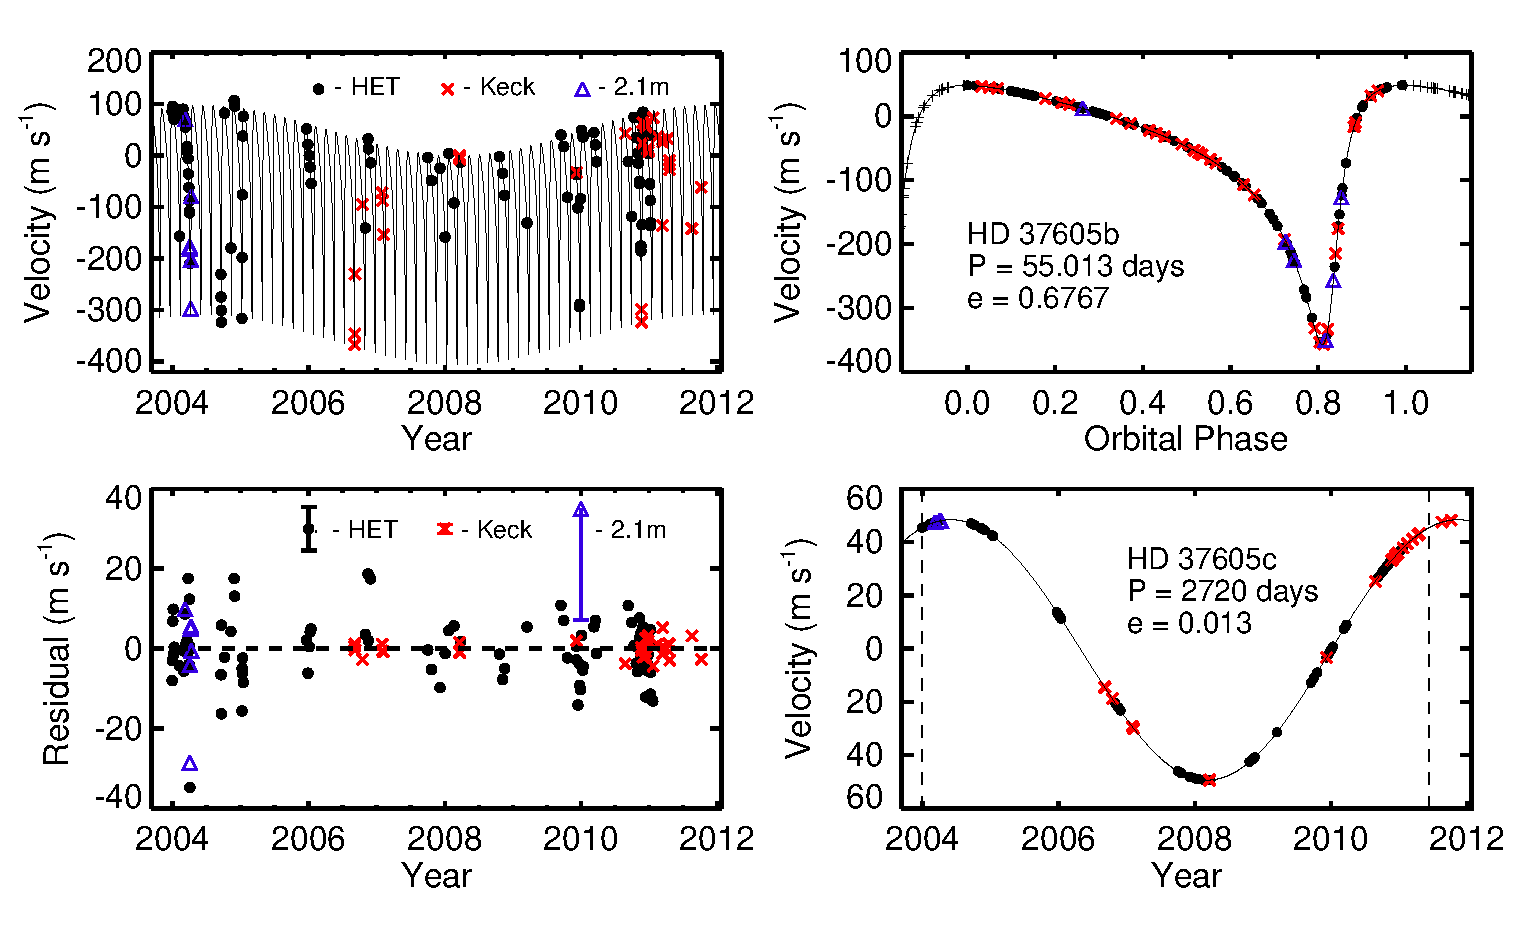
\includegraphics[width=18cm,angle=0]{f1.eps}
%  \subfloat[]{\includegraphics[width=\linewidth,,trim = 0mm -1cm 0mm 0mm]{KissFigures/sfr_8micron.png}}
\begin{figure}
\begin{center}
  \subfloat[]{\includegraphics[width=\linewidth]{KissFigures/direct_8micron.png}}
  \caption{H$\alpha$-derived SFR versus 8.0$\mu$m luminosity, with a line of best fit. Points are color coded by $\LOG{O/H}+12$ metallicity, with a color key to the right of the plot. Metallicity increases with 8.0\micron luminosity and SFR, suggesting that larger galaxies are simply more luminous in all bands (discussed in Section \ref{sec:specific}).\label{simple}}
\end{center}
\end{figure}

\begin{figure}
\ContinuedFloat
\begin{center}
  \subfloat[]{\includegraphics[width=\linewidth]{KissFigures/direct_8micron_dust.png}}
  \caption{Same as Figure \ref{simple}{\bf(a)}, but for 8.0$\mu$m (dust) luminosity}
\end{center}
\end{figure}



%   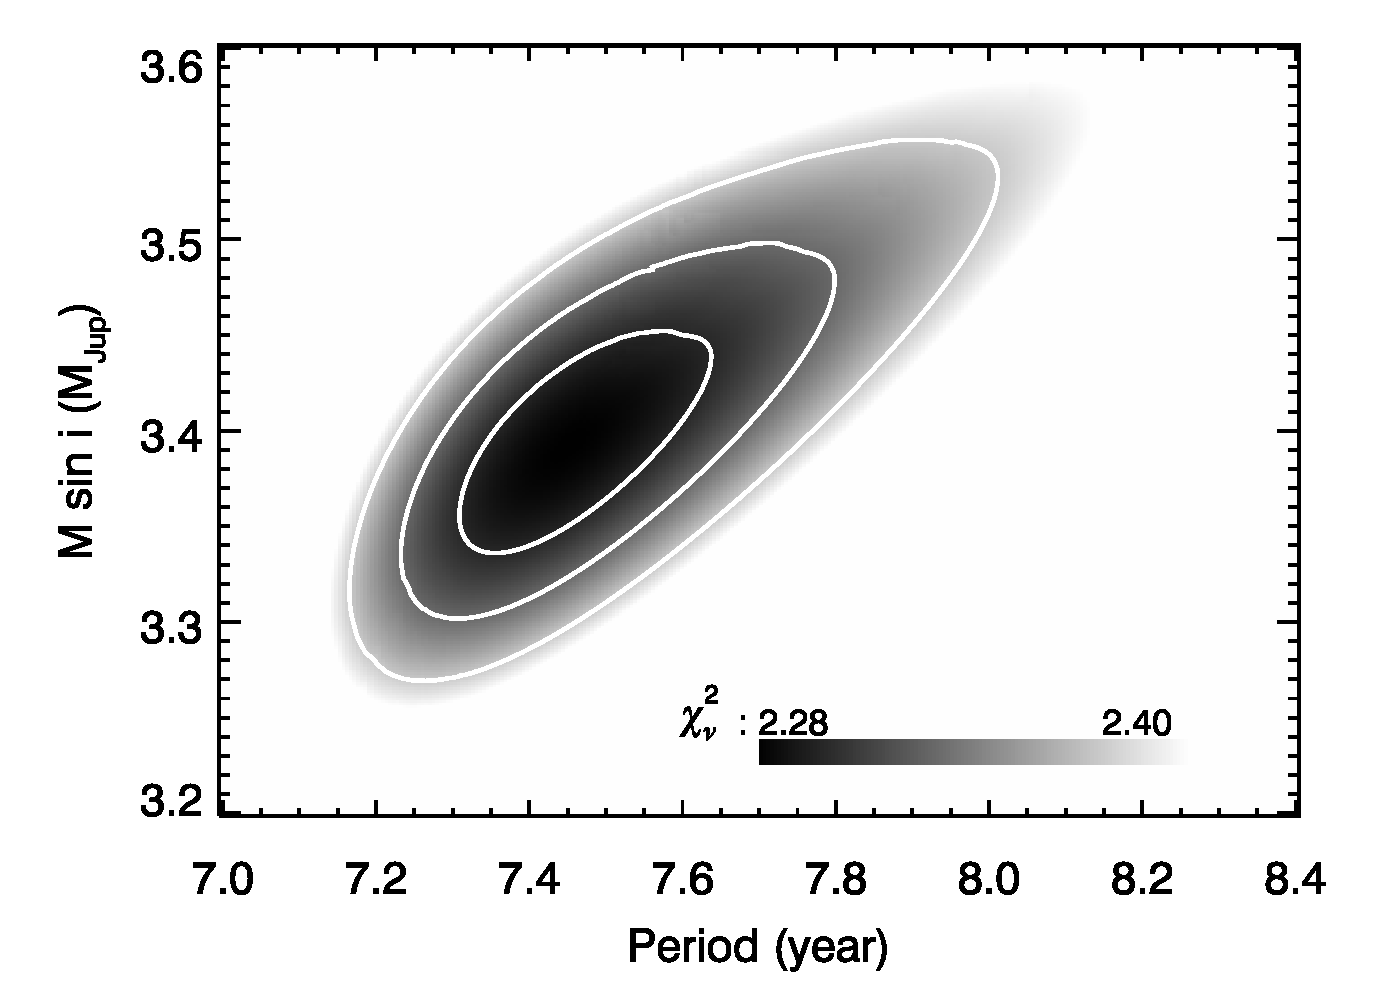
\includegraphics[width=18cm,angle=0]{f2.eps}
\begin{figure}%[T!]
\ContinuedFloat
\begin{center}
  \subfloat[]{\includegraphics[width=\linewidth]{KissFigures/direct_24micron.png}}
  \caption{Same as Figure \ref{simple}{\bf(a)}, but for 24$\mu$m luminosity}
\end{center}
\end{figure}




\begin{figure}%[T!]
\begin{center}
%  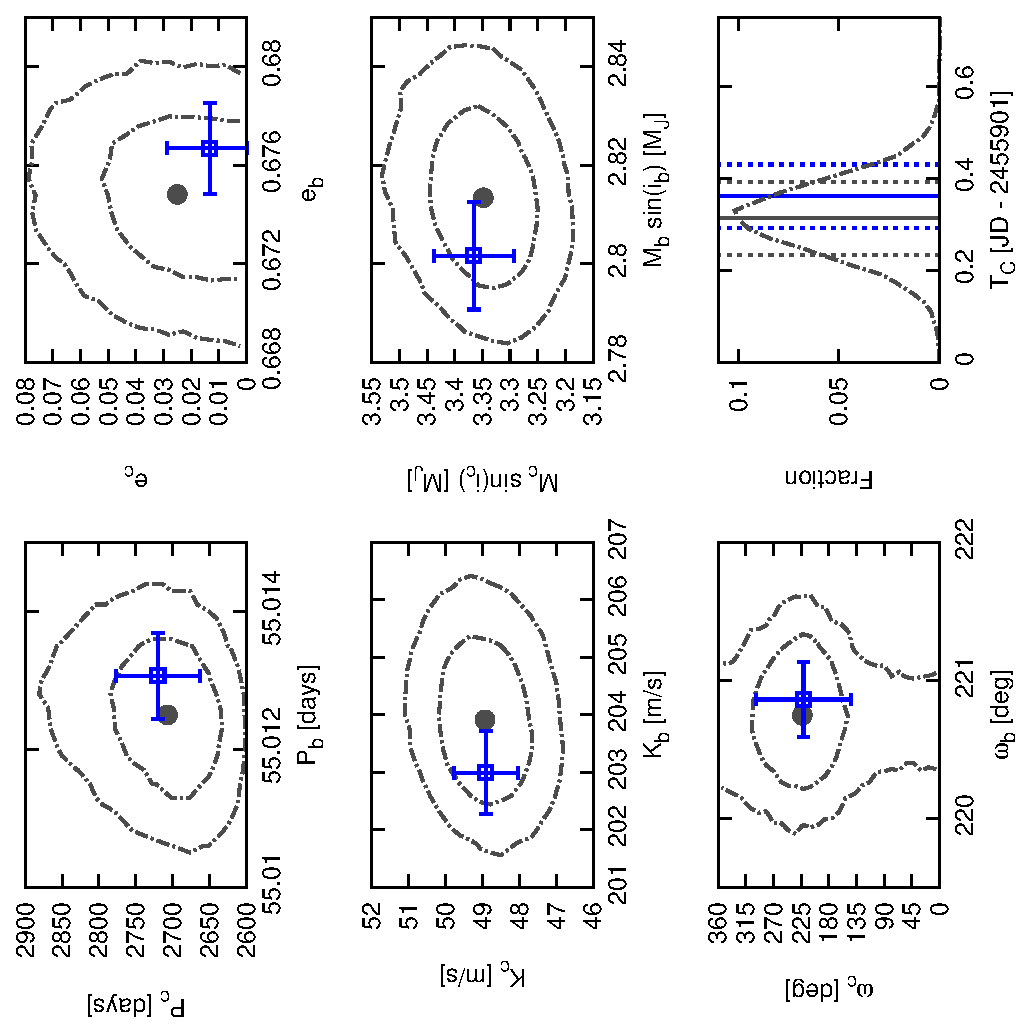
\includegraphics[width=18cm,angle=0]{f3.eps}
  \includegraphics[width=18cm,angle=0]{KissFigures/masses.png}
  \caption{Distribution of stellar masses of the KISS galaxies (black) and Nearby Galaxies (red); note that M31 falls near the upper end of the distribution. Masses are derived from Bw, R, and I band NDWFS photometry \citep{Jannuzi} using mass-to-light relations described in \cite{Bell}.
  }
\label{masses}
\end{center}
\end{figure}


\begin{figure}%[T!]
\begin{center}
%  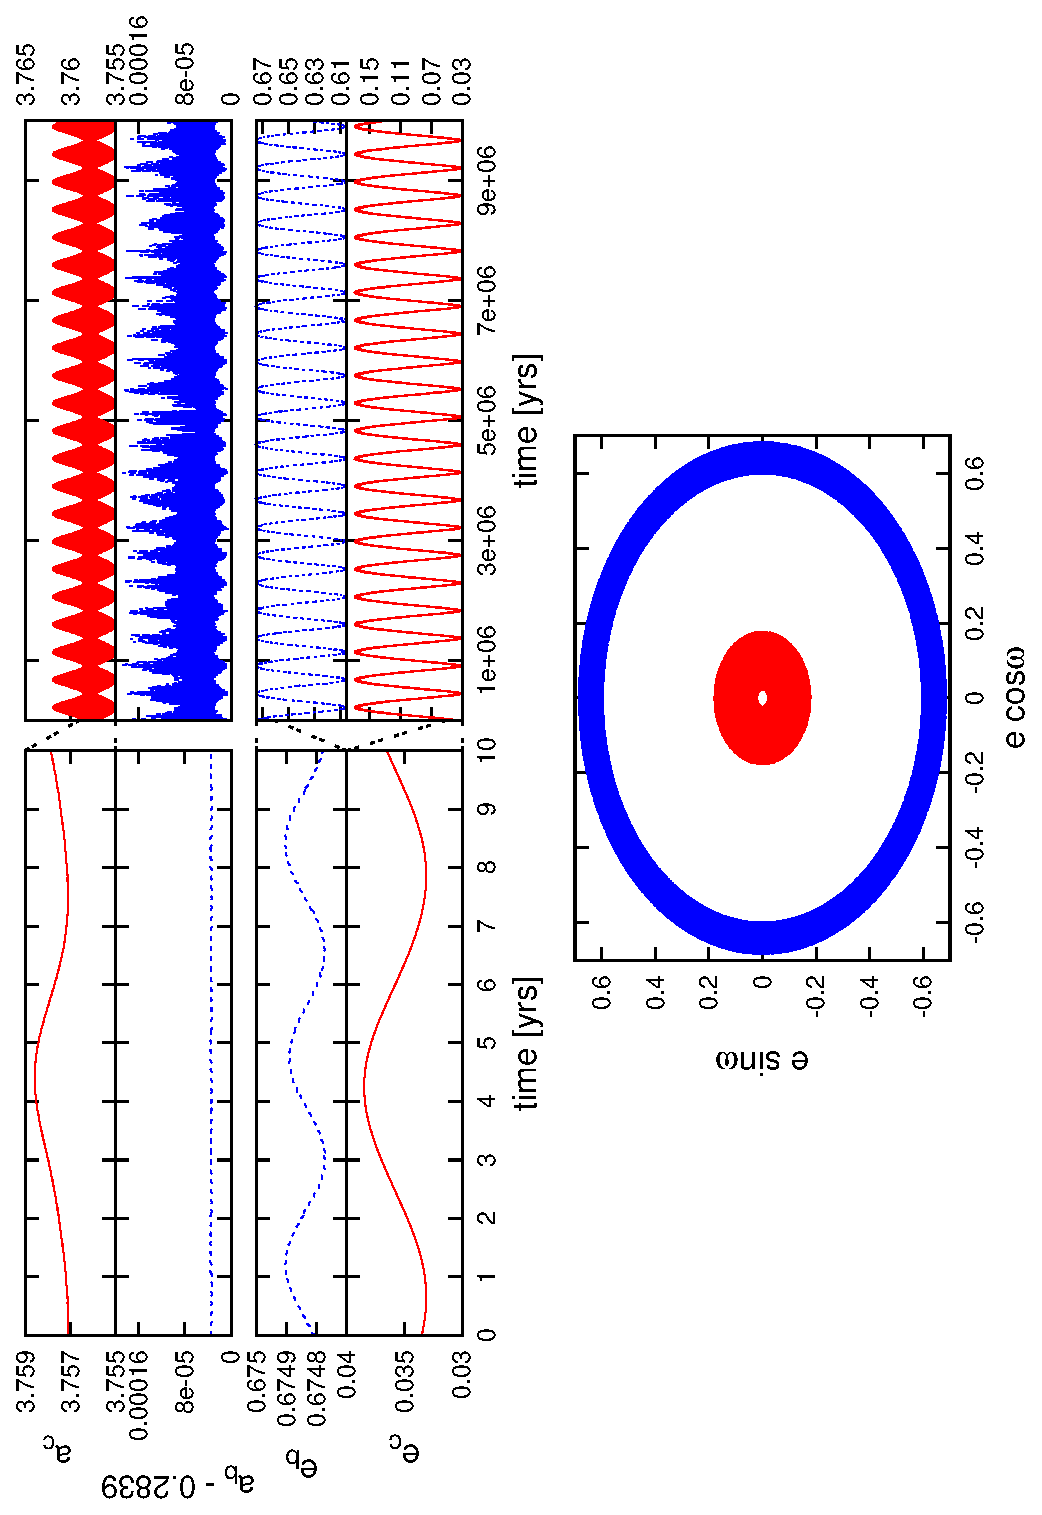
\includegraphics[width=18cm,angle=0]{f4.eps}
  \includegraphics[width=18cm,angle=0]{KissFigures/mass_36micron.png}
 \caption{3.6$\mu$m absolute magnitude versus stellar mass for 81 KISS galaxies. The high correlation justifies the use of 3.6$\mu$m luminosity as a surrogate for mass. Color indicates metallicity, as in earlier figures. Note that there is a strong mass/metallicity trend, but also that there are several 
exceptional galaxies with high metallicities but relatively low masses.}
\label{36micron_mass}
\end{center}
\end{figure}



\begin{figure}%[T!]
\begin{center}
%   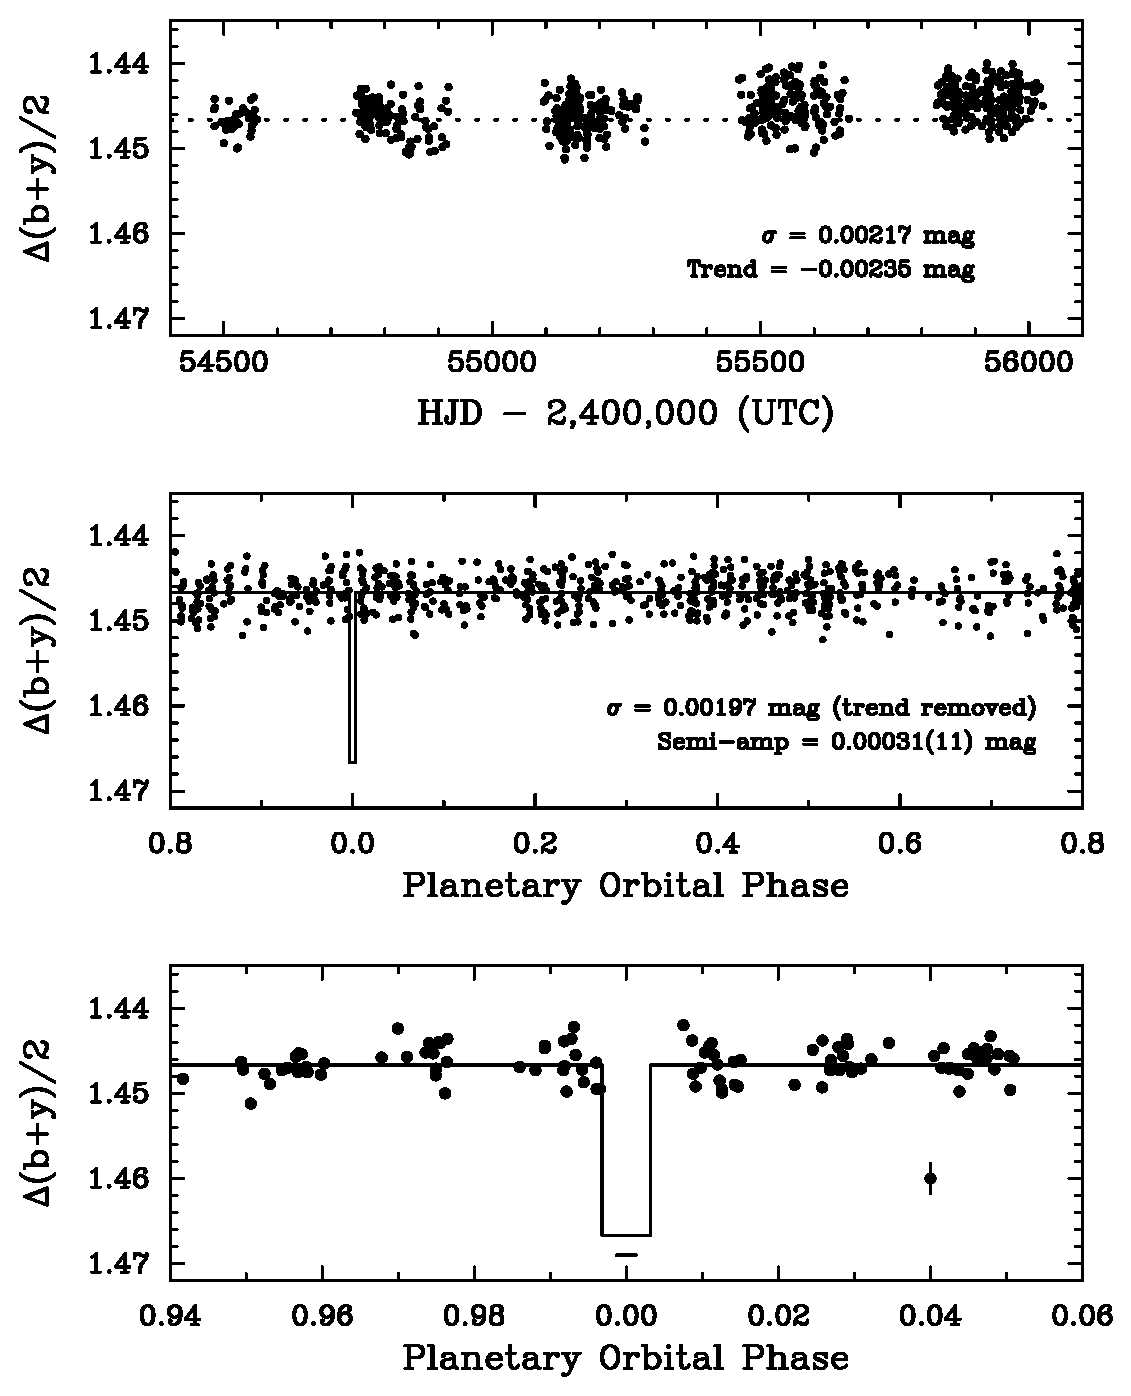
\includegraphics[width=13cm,angle=0]{f5.eps}
   \includegraphics[width=14cm,angle=0]{KissFigures/specific.png}
   \label{sfr_36micron_ir_36micron}

  \caption{
   {\bf (a)} Extinction-corrected H$\alpha$ per 3.6$\mu$m flux versus [3.6$\mu$m]-[8.0$\mu$m] color; essentially SSFR versus specific 8.0$\mu$m luminosity. 
   {\bf (b)} Extinction-corrected H$\alpha$ per 3.6$\mu$m flux versus [3.6$\mu$m]-[24$\mu$m] color; essentially SSFR versus specific 24$\mu$m luminosity per mass. Spearman rank-order analyses of {\bf(a)} and {\bf(b)}, discussed in Section \ref{sec:specific}, indicate no trend whatsoever, implying that SFR to infrared luminosity relations are due to mass/size effects.}


\label{sfr_36micron_ir_36micron}
\end{center}
\end{figure}

\begin{figure}%[T!]
\begin{center}
%  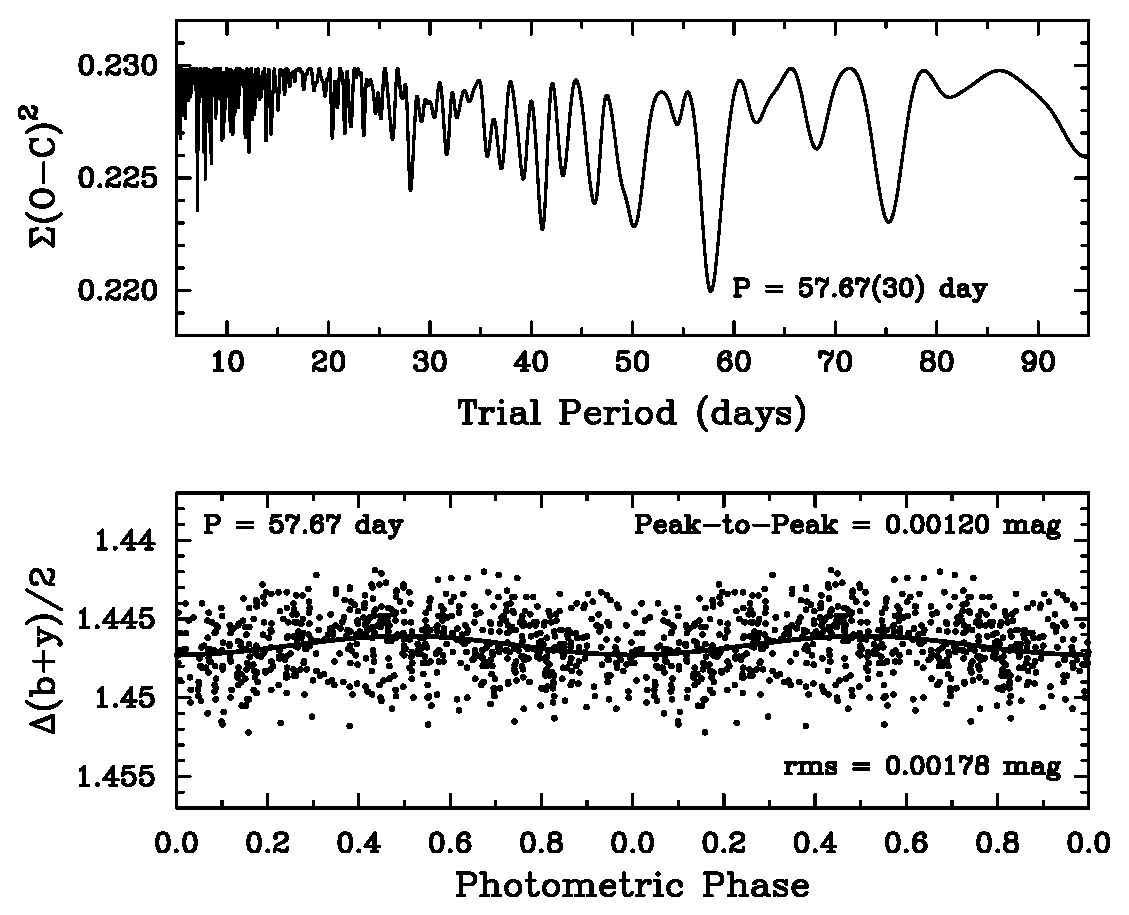
\includegraphics[width=18cm,angle=0]{f6.eps}
  \includegraphics[width=14cm,angle=0]{KissFigures/efficiency.png}
  \caption{
   {\bf (a)} 8.0$\mu$m luminosity per H$\alpha$ luminosity versus 3.6$\mu$m absolute magnitude, with a line of best fit.
   {\bf (b)} 24$\mu$m luminosity per H$\alpha$ luminosity versus 3.6$\mu$m absolute magnitude.
  }
\label{ir_sfr_36micron}
\end{center}
\end{figure}


%\begin{figure}[T!]
%\begin{center}
%\includegraphics[width=17cm,angle=0]{KissFigures/sfr_36micron_36micron.png}
%  \caption{
%  The ratio of H$\alpha$ flux to 3.6$\mu$m flux, a surrogate for star-formation rate per mass, versus 3.6$\mu$m absolute magnitude. Although these points are quite scattered, especially toward the high mass (left) side, I see an overall trend pointing toward higher SSFRs in low mass galaxies.
%  }
%\label{sfr_mass}
%\end{center}
%\end{figure}


